\documentclass[10pt, two column]{article}

\usepackage[utf8]{inputenc}
\usepackage{textcomp}
\usepackage{hyperref}
\usepackage{amsmath}
\usepackage{amsthm}
\usepackage{graphicx}
\usepackage{epigraph}
\usepackage{enumitem}
\usepackage{mathptmx}
\usepackage{times}
\usepackage{listings}

\theoremstyle{definition}
\newtheorem{definition}{Definition}[section]

\lstset{
  basicstyle=\ttfamily,
  columns=fullflexible,
  breaklines=true
}

\title{\huge Phi, a modern successor to Verilog}
\author{Mohamed Gaber\\ The American University in Cairo \and Aya El-Naggar\\ The American University in Cairo}
\date{May 2019}

\begin{document}

\onecolumn
\maketitle
\begin{abstract}
\textbf{Objective:} Develop a new hardware description language focusing on the register transfer level with concise and clear semantics based on the Verilog Hardware Description Language. Method: The language was designed with semantic and syntactic cues from the C and Swift programming languages and the Verilog Hardware Description Language. Conclusion: The language design more accurately reflects the design of the hardware, is less tolerant of ambiguity and is syntactically closer to modern programming languages. Clinical Impact: Because of its simplicity, the language is a great introductory language to digital logic design. It also offers an easy transition for those already writing Verilog.
     
\textbf{Index Terms—hardware description language, verilog, electronic design automation, language design}

\end{abstract}

\tableofcontents

\twocolumn

\section{Introduction}
{\huge\textbf T}he Verilog Hardware Description Language was created in 1984 by Philip Moorby and his team at Gateway Design Automation (now a part of Cadence Design Systems) \cite{threeDecadesofHDL} steadily gained popularity and is currently the dominant modeling language for application-specific integrated circuit (ASIC) design in addition to its considerable presence in field programmable logic array (FPGA) design \cite{foster_2016}. Verilog itself was standardized in 1996 as IEEE Std. 1364-1995 \cite{IEEEstandardHDLbasedonVer_1996}, which was updated multiple times until its latest version in 2006, Std. 1364-2005\cite{IEEEstandardforVerilogHDL_2006}. 
\par

Unfortunately, Verilog is a deeply flawed language by modern standards, being ambiguous and unsafe, with “classic” missteps such as leniency with conversions and other missteps that come from not being designed for purely synthesizable hardware. Many research projects have aimed to design new hardware description languages, however they have tended to either be embedded languages within syntactically alien languages or completely unique research projects that discards most of Verilog’s semantics.\par

This report explores the design and implementation of a new hardware description language based on widely-acknowledged Verilog best practices that does not discard Verilog’s legacy, yet does away with ambiguity, redundancy and makes the syntax closer to the C family of programming languages to appeal to a new generation of hardware designers.

\section{Motivation}
\subsection{Issues with Verilog}
While Verilog was initially designed for both simulation and synthesis \cite{threeDecadesofHDL}, it has been developed solely for simulation for a good portion of its life, and thus has an unfortunate tendency of providing for the description of impossible hardware.\par

As such, Verilog had come to rely on a concept of a “synthesizable subset,”\cite{synthesizableSubset_2017} as there are a lot of features in Verilog that simply cannot be replicated in actual hardware. This is not only limited to constructs that are clearly for simulation, some hardware constructs in Verilog are simply impossible in real life. For example: 
\begin{lstlisting}
always @ (posedge ACLK or negedge ACLK or posedge ARESETn)
\end{lstlisting}

While not inherently faulty, this hardware is not synthesizable as registers tend to only support a single sensitivity, and any more sensitivities would have to be detected using separate hardware. However, as Verilog relies on its “triggers” feature to model sensitive registers, synthesizers are left to deal with this, and some, such as the open source Yosys tool, outright rejecting it.\par

The concept of a “synthesizable subset” is not limited to irreplicable hardware, however, as there are constructs that are purely for simulation. Perhaps the most obvious example is the utilization of software procedural calls. Verilog has a laundry list of function calls that are executed at run time, which are almost impossible to replicate in hardware. It is part of a larger problem with Verilog in general, and it is its general lack of a divide between software and hardware constructs. Between imaginary hardware and literal software, the standard has largely cemented Verilog’s position as a simulation language with limited synthesis capabilities.\par

\subsection{Newer Languages}
These issues have led to various attempts to create other languages to succeed Verilog. These have ranged from university research projects such as University of California at Berkeley’s Chisel\cite{Chisel_2012}, UC at Santa Cruz’s Pyrope\cite{Pyrope} and industry veteran Jon Decaluwe’s MyHDL\cite{MyHDLmanual_2018}.\par

An interesting phenomenon is the development of what has been referred to as an “embedded” hardware description language. At their core, these are libraries written for other programming languages with a desirable syntax and relies on the use of operator overloading and functions to approximate a hardware description language. These do have the advantage of avoiding the syntactic design work, but have the disadvantage of muddying the language semantics with the hardware description semantics, and alienating Verilog users with its syntax.\par 

The most prominent example of this is the Chisel hardware description language. Chisel is embedded into the Scala Programming Language\cite{scalaOverview2004}, and uses its package management for modularization.  It has the added benefit of providing for testbenches to be written in an existing software programming language, which makes more sense as testbenches are, by nature, procedural constructs. Scala addresses a lot of existing problems with Verilog.  A very clear and very separate distinction between run-time and compile-time logic exists by relying on Scala’s robust type system; some types are reserved for run-time logic and others are preserved for compile-time logic. Regardless, these advantages arguably do not outweigh the inherent drawbacks of the use of an embedded language.\cite{Chisel_2012}\par

Another example is MyHDL, which uses the high-level Python programming language. MyHDL clearly differentiates between combinational blocks and sequential blocks using \textbf{@always\_comb} and \textbf{@always\_seq} \cite{MyHDLmanual_2018}, similar to SystemVerilog’s procedural blocks of the same name. However, MyHDL is syntactically and semantically displaced from Verilog, as it utilizes the concept of signals introduced in VHDL\cite{VHDLmanual_2009}. MyHDL has a keyword Signal that represents all signals in a block, and it focuses on the signal going into and out of the block rather than the block itself\cite{MyHDLmanual_2018}.\par

\begin{lstlisting}
Signal(intbv(0)[3:0])
 @always(Clock.posedge)
 def logic1():
  Q.next = concat(Q[2:0],SI)
 return logic1
\end{lstlisting}
\begin{center}
\textit{MyHDL code}
\end{center}

Some others are supersets of Verilog, the most popular being SystemVerilog, which has become so popular in recent years that the synthesizable subset of SystemVerilog is de-facto Verilog itself. SystemVerilog introduces powerful new software features for verification, which has paid off as SystemVerilog continues to be the most popular language for simulation and verification of both ASIC and FPGA designs\cite{foster_2016}. However as a superset of Verilog it continues to inherit many of its problems.\cite{IEEEstandardforVerilog_UHD_S_VL_2005}\par

Lucid is an interesting experiment being a language loosely based on Verilog, much like the language this paper is concerned with, as it does not only show how the building blocks interact together but it also shows what are the building blocks very explicitly. In the given example Lucid mentions \textbf{dff pipe[4]} which are easily inferable to mean 4 D flip-flops. Lucid also makes the representation of D flip-flops very clear by using .d and .q to represent the inputs and outputs. However, other limitations include Lucid's continued dependence on procedural blocks, as well as some strict opinionation on variable naming\cite{withMojoAndLucid_2017}.\par

\begin{lstlisting}
dff pipe[4] (.clk(clk));
   var i;
     always {
       pipe.d[0] = serial_in;
       serial_out = pipe.q[3];
       for (i = 1; i < 3; i++)
         pipe.d[i] = pipe.q[i-1];
\end{lstlisting}
\begin{center}
\textit{Lucid code}
\end{center}

There are some languages that are built from scratch like Pyrope, however they tend to ignore Verilog's legacy altogether: Pyrope is particularly removed from Verilog syntactically and semantically even more so\cite{Pyrope}. That is not to say these languages do not have their merits, as Pyrope prides itself on being fully synthesizable. For newcomers this might not be a problem, however as the industry is very dependent on Verilog, it can be rather difficult to move to a completely different paradigm.\par

\subsection{Design Goals for Phi}
Phi’s primarily design goal is the creation of a hardware description language that is syntactically and semantically more concise than Verilog, yet one that embraces Verilog’s legacy by continuing to be ultimately structurally, semantically and syntactically similar to the Verilog Hardware Description Language.\par

This can be boiled down to four essential goals:
\begin{enumerate}[label=\alph*)]
\item Unambiguous
\item Fully synthesizable
\item Closer to the C family of languages to appeal to newcomers
\item Close to Verilog semantically to not alienate its veterans.
\end{enumerate}

These goals should be able to culminate in a language that is simple to use, more efficient in a production environment, easier to learn by newcomers but not a jarring transition for existing Verilog users.

Phi's initial design involved field testing by the author of this people responsible for much of the research into contemporary languages independently of the language's designer.

\section{Design Process}
As a successor to Verilog with inspirations from the C-family of languages, it was clear Phi was going to be developed as a derivative language rather than one that is designed from scratch. Semantically, the obvious choice was Verilog, as it could then be cut to size from the verbosity. Syntactically, the Swift Programming Language was chosen, as it had a modern, expressive yet concise take on C and C++’s syntax \cite{swiftProgLang2019}.\par
 
Many elements, such as the general code organization, have been retained from Verilog. There is a single top module that instantiates other submodules, where this module is then used for simulation or synthesis.\par 

\begin{figure}
  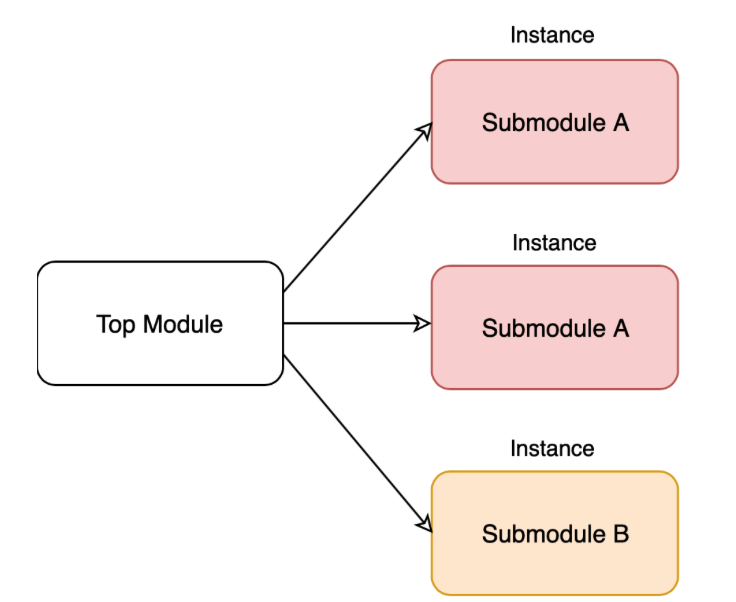
\includegraphics[width=\linewidth]{module_hierarchy.png}
  \caption{\textit{Module Hierarchy in Verilog and Phi}}
  \label{fig:module_hierarchy}
\end{figure}

Perhaps the most significant semantic departure for Phi is the lack of a software type system. A type system has never particularly made sense in hardware, as all values are bit-vectors where each wire can only be off or on. In other hardware description languages, it seems that trajectory is to introduce stricter typing. While it improves code safety in software, in hardware such behavior is counterproductive. In Phi, the operators decide how the bit-vectors should behave, similar to assembler languages. Arithmetically, they behave as integers. Inspired by ECMAScript\cite{ECMAScript_2018}, the one operation where the sign matters on bit-vectors, the right shift, was migrated to Phi, where it has similar behavior.\par

This has also affected Phi’s syntax import from Swift, as Swift’s typing syntax did not translate very well. Swift used var and let to denote declaration and an extra identifier for type expressions. The concept of types doesn't exist in Phi, and thus Phi reverted to C-style declarations of type, then variable name.\par 

The “types” in said situation refer to “Var”, “Register”, "Latch" and “Wire”, where the first indicates software expressions evaluated at compile/elaboration time, and the latter three are hardware constructs to be simulated or synthesized, i.e., "run time" expressions. This is to satisfy the goal of a strict software/hardware divide.\par

This strict software/hardware divide also allows for initially more cumbersome definitions in Verilog to become less so, such as declaring arrays of components. What required the Verilog generate block- essentially metaprogramming, is now idiomatic to Phi as now components can now be declared in arrays and hooked separately. For example:\par

\begin{lstlisting}
genvar i;
for (i = 0; i < 10; i = i + 1) begin
    Example example(
        .a(a[i]),
        .b(b[i]),
        .q(q[i]),
        .r(r[i])
    );
end

Example example[10]
for i in 0..9 {
    example[i](
        a: a[i],
        b: b[i],
        q: q[i],
        r: r[i]
    )
}
\end{lstlisting}
\begin{center}
\textit{Instantiating an array of modules in Verilog (top) and Phi (bottom)}
\end{center}

What does have the potential to create a difference in a hardware description language is bus width safety. Unlike Verilog, Phi is strict about bus widths, and these requirements may not be waived. Phi will not automatically extend nor prune expressions to fit a specific bus width. This rule is universal: for example, even an expression as trivial as \textbf{1b1 + 1b1 + 1b1} would be incorrect, as the first two result in a two-bit wide expression that would be incompatible with the third one-bit wide expression. Additionally, all if conditions can only be one bit.

Incidentally, numbers in Phi are encouraged to specify a width and a base, for example \textbf{30xABC} would declare a 30-bit integer with the unsigned decimal value of 48879. Numbers declared without a width and base are 32-bit and decimal by default, but their use is discouraged outside of ranges.\par

Perhaps the most significant semantic departure in Phi relates to the function of storage objects such as latches and registers. Phi represents these as special structures with properties accessible via the dot notation, e.g. \textbf{register.clock}, that influence the behavior of an otherwise abstract object. Registers have four such properties: \textbf{.data, .reset, .clock, and .enable}, while latches have three: \textbf{.condition, .data, and .enable}. The Register and Latch objects are roughly analogous to D flip-flops and D latches: the Registers write the value of .data to themselves when the .clock signal is high, and resets asynchronously when the .reset signal is high. The .enable signal is optional, and if driven at all, the register will prevent any writes to itself as long as the .enable signal is low. Assigning to a register simply sets its reset value (i.e. the value written when .reset is high,) and the register's identifier is usable to obtain the current value of the register. The same goes for latches, albeit the only difference is the .data value is written when both .condition and .enable are driven high. As writing separate .clock, .reset and .enable assignments for every Register and/or Latch would become repetitive, \textbf{annotations} were introduced to allow for the setting of a specific input signal to be the clock, reset, condition or enable for all Registers and/or Latches in a module. For example, declaring an input port named "clk" as \textbf{clk: @clock Input} sets clk to be the .clock signal for all registers in a module, unless explicitly otherwise specified for a specific module.\par

\begin{figure}
   \resizebox{0.5\linewidth}{!}{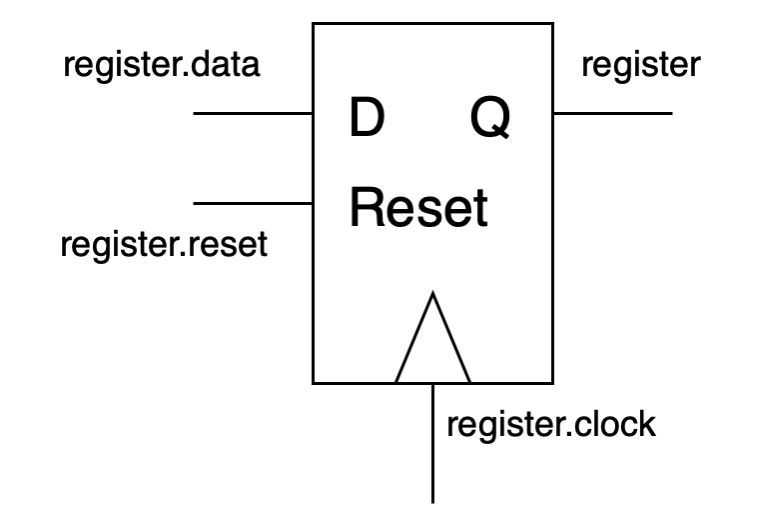
\includegraphics{register_in_phi.png}}
  \caption{\textit{A Register in Phi. Registers in Phi are based on D flip-flops.}}
  \label{fig: a register in Phi.}
\end{figure}

Phi embraces the concept of perpetuity in hardware. As actual hardware, with the possible exception of FPGAs, do not have an “initial” state, and so it is beneficial that all elements of Phi execute in perpetuity. Therefore, it has been decided that Phi would do away with synchronous procedural blocks entirely. Attempting to translate the semantics of Verilog triggers to something more synthesizable proved a futile effort: it would always boil down to a way to specify clocks and resets for a set of registers anyway.

Phi has thus transitioned to a model where procedural blocks are only used to model combinational logic. The actual writing to the register is black-boxed to the designer, as they should be at the register-transfer level. Phi does not support lower level modeling of hardware. Being that registers now write perform writes independently, registers can now no longer be assigned to with blocking or non-blocking semantics: using the = operator sets the value of the register when reset.\par

The asynchronous procedural blocks are known in Phi as the \textbf{comb} blocks. At a basic level, the \textbf{comb} block is similar to the \textbf{always\_comb} block in Verilog, with the key distinction being that in Phi, there are a set of rules in place to ensure the expressions are truly combinational:

\begin{enumerate}[label=\alph*)]
\item No declarations can occur inside comb blocks.
\item If an object is assigned to inside an comb block, the assignment must occur under all conditions.
\item A wire cannot be a function of itself, i.e. it cannot depend on its own value.
\end{enumerate}

\begin{lstlisting}
comb {
   if (y) {
       a = 32b0
   } else {
       a = 32xBAD
   }
}
\end{lstlisting}
\begin{center}
\textit {A comb block in Phi.}
\end{center}

Another area where Phi has changes when compared to Verilog is procedural system calls. Verilog system calls can occur at run-time, but Phi firmly restricts these features to compile time and forces them to return a bit-vector. There are five such functions: \textbf{abs, log, pow, fromFile, and interpretFromFile}: the last one being the most similar to Verilog's popular \$readmemh and \$readmemb procedural system calls.

There are other numerous small semantic tweaks. This includes namespacing, which allows modules or declarations inside a module to exist under a namespace where they would later have to be accessed with the dot notation popularized by C. It allows multiple modules to exist with the same name, so long as they are properly namespaced. On the topic of modules, Phi also defines interfaces in the vein of Java’s 
interfaces and Swift’s protocols, which would define a set of input ports that instantiators would have to drive and a set of output ports that the compliant module would have to drive. This is especially useful when developing intellectual properties for use with buses, which do tend to mandate certain port names and/or widths. We have also elected to introduce a \textbf{mux} expression that is more general than a ternary operator: it replaces a binary condition with a full selection line and more than two possible outcomes.\par

\begin{lstlisting}
readData = mux read (1b0: 32b0, 1b1: data)
\end{lstlisting}
\begin{center}
\textit {A mux block in Phi.}
\end{center}

There are also a number of syntactic tweaks, the most obvious of which is the substitution of begin and end tokens with braces. As shown in the instantiation of arrays, the C-style for loop has been abandoned in favor of the \textbf{for in} loop used in more modern C-family languages. Imperative software loops are harder to deal with when all values are constants. Ranges have had their syntax slightly tweaked, now using the .. operator from Perl and Ruby for familiarity's sake. Semicolons were made optional in order to become slightly more in line with Swift.\par

\begin{lstlisting}
module Counter(
   clock: @clock Input,
   reset: @reset Input,
   output: Output[31..0]
) {
   Register[31..0] store = 32b0
   store.data = store &+ 1
   output = store.data
}
\end{lstlisting}
\begin{center}
\textit{A typical Phi module under this design}
\end{center}

Some challenges persist with designing Phi: for example, whether to support a C-style preprocessor or a module system similar to Java or Swift would. Another area of interest is idiomatic decoding of arrays of components; currently, all array and range accesses in Phi are software expressions, which is not the case in Verilog cod. As some simple expressions involving arrays can be synthesize, but not the majority, introducing this feature to Phi would be a bit of a tall order.

\section{Implementation}

As a result of the limited labor resources, Phi was implemented using well documented industry-standard tools, with almost no custom components.\par

Phi was initially implemented in the classic duo of Unix compiler implementation: Lex and Yacc. Because these tools are a part of the UNIX® specification \cite{openGroupBaseSpecif_2018}, supporting these tools would have made the compiler very portable across multiple platforms. However, this has introduced many limitations stemming from the fact the compiler was written in C++, which is not a part of the Unix specification. While it is possible to have implemented this compiler in C, time constraints and the team’s own development experience could not accommodate that, and it was quickly switched over to GNU Flex and GNU Bison, as both tools do have limited support for C++.\par

Bison’s C++ support is impressive; but flawed: on one hand, it generates a full “Parser” class that fully encapsulates its functionality, but on the other hand, its reliance on unions has lead to some safety issues with the compiler. Flex did not fare as well, generating code that was invalid when operated in C++ mode. Instead of GNU flex, which has non-functional C++ support, we elected to use an open source tool named RE-flex by Genivia Inc\cite{reflex}. RE-flex was found to be a better fit for this project than flex: it is written in and generates C++, has a speed advantage and supports Unicode, which is an advantage for some markets such as China.\par

There are, nevertheless, some limitations with the current implementation of the compiler: the most challenging of which is parameterization, as Phi modules are instantiatable by Verilog modules: some values that incorporate parameters would be unknown to Phi at compile time. An automated theorem prover or similar would have to be included with the Phi compiler to rectify this issue, and verify widths in terms of variables. Other key features missing include the checks on multiplexer and switch statement exhaustiveness, as well as the checks on comb blocks. There are a number of smaller features missing purely due to time constraints and not implementation challenges, but the compiler acts as a proof of concept for the hardware description language.\par

\section{Comparison}
To show the degree to which Phi is an improvement over Verilog, we decided to implement some simpler modules written by students for assignments. We felt that the module that best showcases some of the improvements in Phi is an assignment about successive approximation registers. Note that for both, an \textbf{EdgeDetector} module is assumed to exist.

\begin{lstlisting} [
    basicstyle=\tiny
]
module SuccessiveApproximationControl(clk, reset, go, cmp, valid, result, value, sample);

input clk, go, cmp, reset;
output [15:0] value;
output [15:0] result;
output reg valid;
output reg sample;

wire actuallyGo;

reg [15: 0] successiveApproximationRegister;
reg [15: 0] position;
reg [7: 0] waiting;
reg running;

assign value = successiveApproximationRegister;
assign result = successiveApproximationRegister;

EdgeDetector goDetector(.clk(clk), .reset(reset), .go(go), .actuallyGo(actuallyGo));

always @ (posedge clk or posedge reset) begin
    if (reset) begin
        valid <= 1'b0;
        running <= 1'b0;
        sample <= 1'b0;
        waiting <= 8'b0;
        successiveApproximationRegister <= 16'h0;
    end
    else if (actuallyGo && !running) begin //Nothing is running
        running <= 1'b1;
        sample <= 1'b1;
        valid <= 1'b0;
        successiveApproximationRegister <= 16'h8000;
        waiting <= 8'd4;
        position <= 16'h8000;
    end
    else if (running && waiting) begin //Running, waiting
        waiting <= waiting - 1;
    end
    else if (running && position) begin 
        sample <= 0;
        // Intentionally blocking for the next set of lines
        if (cmp) begin
            successiveApproximationRegister = successiveApproximationRegister ^ position;
        end
        position = {1'b0, position[15:1]};
        successiveApproximationRegister = successiveApproximationRegister | position;
    end
    else if (running) begin
        valid <= 1'b1;
        running <= 1'b0;
    end
end

endmodule
\end{lstlisting}
\begin{center}
\textit{A successive approximation register written for a student assignment. A number of unsafe or difficult to synthesize constructs are utilized.}
\end{center}

As can be seen, a degree of confusion at blocking and non-blocking assignments and registers versus wires had let to a mixing of blocking and non blocking assignments inside the procedural block.

In Phi, the situation is far simpler:

\begin{lstlisting} [
    basicstyle=\tiny
]
module SuccessiveApproximationControl(clk: @clock Input,
    reset: @reset Input,
    go : Input,
    cmp: Input,
    valid: Output,
    result: Output[15..0],
    value: Output[15..0],
    sample: Output
) {
    Register[15..0] sar = 16d0
    Register[15..0] position = 16d0
    Register[7..0] waiting = 8d0

    Register running = 1d0
    Register doSample = 1b0
    Register isValid = 1d0

    value = sar
    result = sar
    sample = doSample
    valid = isValid

    Wire actuallyGo
    Wire[15..0] positionShifted

    EdgeDetector goDetector(clk: clk, reset: reset, go: go, actuallyGo: actuallyGo)

    comb {
        running.data = running
        doSample.data = doSample
        isValid.data = isValid
        sar.data = sar
        waiting.data = waiting
        position.data = position

        if actuallyGo & ~running {
            running.data = 1b1
            doSample.data = 1b1
            isValid.data = 1b0
            sar.data = 16x8000
            waiting.data = 8d0
            position.data = sar.data
        } else if running & waiting {
            waiting.data = waiting &- 1
        } else if running & (position != 16b0) {
            doSample.data = 1b0
            position.data = {1b0, position[15..1]}
            sar.data = mux cmp (1b1: sar ^ position, 1b0: sar) | position.data
        } else if running {
            isValid.data = 1b1
            running.data = 1b0
        }
    }
}
\end{lstlisting}
\begin{center}
\textit{The same SAR implementation rewritten in Phi.}
\end{center}

As a result of Phi's rethinking of registers and procedural blocks, users are now free to assign to any wire in a blocking manner, so long as Phi's three checks are obeyed, which is true of this comb block. As all assignments here are blocking, the most egregious part in the Verilog implementation is solved quite nicely, where both position and position.data's values can be used in sar.data's complex expression, which is not easily possible in Verilog as you cannot assign to wires in procedural blocks.

\section{Conclusion}
While there are a few implementation flaws remaining to iron out, as a language Phi remains simple and attractive to newcomers, and yet any industry veteran should be able to quickly realize its design around informal Verilog best practices.\par

Phi does achieve its goal of eliminating ambiguity: the elimination of procedural blocks in particular and its reliance on a more structural style of modeling provides for a pure and transparent RTL flow in comparison to other languages.\par

Phi's features also focus on the development of hardware in an era of tightly integrated and possibly even open source electronic design automation tools. The compiler is not built to be standalone, it is also built to integrate with other tools- starting from the error reporting providing short strings that can be localized independently.\par

\section*{Appendix}
Phi is available as of the time of writing at \url{https://github.com/donn/Phi}. The full specification is available under the folder "Specifications". Usage instructions is available in Readme.md in the root of the repository. The Phi compiler was tested on  Apple macOS and GNU/Linux (Ubuntu 19.04).

The source code for this research paper is available under the folder "Paper". All code used in the comparison, including the testbench, is available in the same folder.

The testing examples/formative suite used in the evolution of the language's design are available at \url{https://github.com/donn/Phi-Examples}.

\section*{Acknowledgment}
We would like to acknowledge Professor Mohamed Shalan of the American University in Cairo for his consistent input on the design of the Phi Hardware Description Language, and Professor Sherif Aly of the same university for supervising and advising the research aspect of this project.

\bibliography{refs}
\bibliographystyle{ieeetr}

\end{document}
